\documentclass[a0]{sciposter}
%\usepackage[latin1]{inputenc}
\usepackage[T1]{fontenc}
\usepackage[utf8]{inputenc}
\usepackage{textcomp}
%\usepackage{hyperref}
\usepackage{lipsum}
\usepackage{epsfig}
\usepackage{amsmath}
\usepackage{amssymb}
\usepackage{multicol} 
\usepackage{graphicx,url}
\usepackage[english]{babel}   
\usepackage[svgnames]{xcolor}
\usepackage{empheq}
\usepackage[most]{tcolorbox}
\usepackage{anyfontsize}
\usepackage{t1enc}
%\usepackage[utf8]{inputenc} 
%\usepackage{fancybullets} 



\newtcbox{\mymath}[1][]{%
    nobeforeafter, math upper, tcbox raise base,
    enhanced, colframe=blue!30!black,
    colback=blue!30, boxrule=3pt,
    #1}


 \definecolor{qq}{rgb}{.6, 0.0, 0.99}
 
\renewcommand{\familydefault}{\rmdefault}
%\renewcommand{\titlefont}{\rmfamily}


%\setlength{\topmargin}{-4.5pc}
%\setlength{\rightmargin}{-8.5pc}
%\setlength{\leftmargin}{200.5pc}
%\setlength{\textheight}{1900mm}
%\setlength{\oddsidemargin }{-4.0pc}
\setlength{\textwidth}{790mm}
\setlength{\textheight}{1450mm} 

\setlength{\headheight}{0pt}
\setlength{\headsep}{-10.0pt}
\setlength{\topmargin}{-100.0pt}
\setlength{\oddsidemargin}{-80.0pt}

\institute 
{Jagiellonian University in Kraków}
%Nome e endereço da Instituição

%\email{asyrwid@gmail.com}
% Onde você coloca os emails dos integrantes


%\date is unused by the current \maketitle


% Exibe os logos (direita e esquerda) 
% Procure usar arquivos png ou jpg, e de preferencia mantenha na mesma pasta do .tex
%%%%%%%%%%%%%%%%%%%%%%%%%%%%%%%%%%%%%%%%%%%%%%%%%%%%%%%%%%%%%%%%%%%%%%%%%%%%%%%%
%%% Begin of Document



\begin{document}
%define conference poster is presented at (appears as footer)

%\LEFTSIDEfootlogo  
% Uncomment to put footer logo on left side, and 
% conference name on right side of footer

% Some examples of caption control (remove % to check result)

%\renewcommand{\algorithmname}{Algoritme} % for Dutch

%\renewcommand{\mastercapstartstyle}[1]{\textit{\textbf{#1}}}
%\renewcommand{\algcapstartstyle}[1]{\textsc{\textbf{#1}}}
%\renewcommand{\algcapbodystyle}{\bfseries}
%\renewcommand{\thealgorithm}{\Roman{algorithm}}


\vspace{-0.5cm}
\center
\includegraphics[width=6.0cm]{ujlogo.pdf}	

\vspace{0.5cm}

%\begin{minipage}[l]{0.9\textwidth}
%\begin{flushleft}
\color{DarkBlue}
\center
\textbf{\Huge{Bayes' theorem and fluctuation theorems}
}

\color{black}
\vspace{0.9cm}

\textbf{\Large{Author:}} \Large{\underline{Micha\l{} Mandrysz}, \ Jagiellonian University in Krak\'{o}w}
\vspace{0.6cm}

% University/organization
%\end{flushleft}
%\end{minipage}
%\begin{minipage}[r]{0.1\textwidth}
%\includegraphics[width=6.0cm]{ujlogo.pdf}
%\end{minipage} 

%\begin{minipage}[b]{0.1\linewidth}
%\includegraphics[width=2.5cm]{ujlogo.pdf} % Logo or a photo of you, adjust its dimensions here
%\end{minipage}
%\begin{minipage}[b]{0.127\linewidth}
%\includegraphics[width=3.5cm]{ubial.jpg} % Logo or a photo of you, adjust its dimensions here
%\end{minipage}
%\begin{minipage}[b]{0.11\linewidth}
%\includegraphics[width=2.2cm]{ifpan.png} % Logo or a photo of you, adjust its dimensions here
%\end{minipage}



%\vspace{1.0cm}

%%% Begin of Multicols-Enviroment


%%% Abstract
%\begin{abstract}
%\medium
Using Bayes' theorem we present a simple and general model which allows us to generate distributions of change in entropy between two macroscopic states. Obtained results are with agreement with the Second Law of thermodynamics, favouring decrease in the number of macroscopic states (keeping the number of microscopic states constant) and thus increasing the number of microscopic realisations of the surviving macrostates.
Due to the close resemblance of our expression to the fluctuation theorems we discuss its relation to Crooks Fluctuation Theorem. Surprisingly, the distributions obtained during experimental verification of Crooks relation on RNA strands follow closely the distributions obtained from our Bayesian relation.
%\end{abstract}

\begin{multicols}{3}


%====================================================================================================================================
%====================================================================================================================================
%====================================================================================================================================
%====================================================================================================================================

%%% Introduction
\section{Bayesian model for a generic isolated physical system}
\normalsize
\begin{flushleft}
Consider a generic statistical mechanical system with a \textbf{fixed number of microstates}, evolving under deterministic, microscopic equations of motion. 
\begin{itemize}
	\item $t_0$, $t_1$ - initial and final times
	\item $\{A_i\}, \{B_j\}$ - sets of initial and final macrostates
	\item $N_A, N_B$ - numbers of initial and final macrostates
	\item $M_i, N_j$ - numbers of microscopic realizations of $i$ initial and $j$ final macrostates.
	\item $K_{ij}$ - number of initial microstates of macrostate $A_i$ flowing into the final macrostate $B_j$, as illustrated on figure \ref{Fig1}.
\end{itemize}

\end{flushleft}
\vspace{-0.5cm}
\begin{minipage}[b]{20.0cm}
\centering
\begin{figure}[ht!]
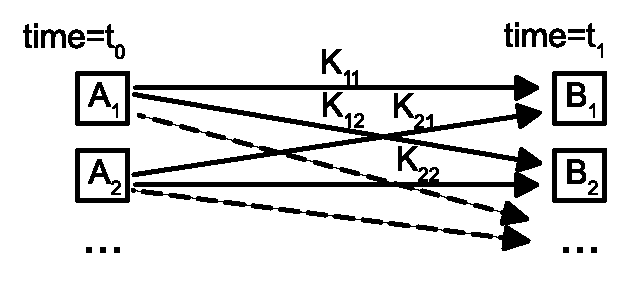
\includegraphics[width=20.0cm]{figure1.eps}
\caption{Transitions between macrostates ${A_i}$ and macrostate ${B_i}$ dictated by the 'transition' matrix $K_{ij}$.}
\label{Fig1} 
\end{figure}
\end{minipage}
\begin{flushleft}
\vspace{-1.0cm}
The probability of the forward transition:
\begin{equation}
\label{ForwardProb}
  P(B_j|A_i)= \frac{K_{ij}}{M_i}.
\end{equation}
However, the probability of the time reversed case (post-diction) is given by the \textit{extended Bayes theorem}:
\begin{equation}
  P(A_i|B_j)=\frac{P(B_j|A_i)P(A_i)}{\sum_k P(B_j|A_k)P(A_k)}.
\end{equation}

Having no a priori knowledge about the initial macrostates, each of them is equally probable $P(A_i)= 1/N_A$, getting:

\begin{equation}
\begin{aligned}
  P(A_i|B_j) &= \frac{K_{ij}}{M_i} P(A_i) \left( \sum_k \frac{K_{kj}}{M_k}P(A_k) \right)^{-1}\\
  &= \frac{K_{ij}}{M_i} \left( \sum_{k} \frac{K_{kj}}{\sum_m K_{km}} \right)^{-1},
\end{aligned}
\end{equation}
\vspace{0.5cm}
\begin{tcolorbox}[colframe=green!500!white,colback=white!50!white,boxrule=3pt]
The conditional probabilities $P(B_j|A_i)$ and $P(A_i|B_j)$ are entirely different in nature - the first represents a prediction, but the second is a post-diction. There is no symmetry between assumptions and assertions in conditional probability calculus.
\end{tcolorbox}
\vspace{0.5cm}
The ratio of prediction and postdiction:

\begin{tcolorbox}[colframe=red!500!white,colback=white!50!white,boxrule=3pt]
\begin{equation}
\label{MacrostatesPRatio}
  \frac{P(B_j|A_i)}{P(A_i|B_j)}= e^{\ln{\sum_{k} \frac{K_{kj}}{\sum_m K_{km}}}}.
\end{equation}
\end{tcolorbox}
\vspace{0.5cm}

Since, the number of microstates doesn't change (energy does not flow in or out) -- the natural interpretation of the term in the exponent is the configurational (internal) entropy change: 
%\vspace{0.5cm}
\begin{equation}
\label{ConfEntropy}
  \Delta S = \frac{\Delta E - \Delta F}{T} \implies -\frac{\Delta F}{T}
\end{equation}
\vspace{-0.5cm}
\begin{tcolorbox}[colframe=green!500!white,colback=white!50!white,boxrule=3pt]
\begin{equation}
\Delta S_{conf} /k_B = \ln{\sum_{k} \frac{K_{kj}}{\sum_m K_{km}}} = - \beta \Delta F
\end{equation}
\end{tcolorbox}
\vspace{-0.5cm}
In the limiting case of \textit{one} initial macrostate we recover the \textit{Boltzmann entropy}:
\vspace{-0.5cm}
\begin{equation}
\Delta S_{conf} /k_B = \ln{\sum_{k} \frac{K_{kj}}{\sum_m K_{km}}} \stackrel{\#k=1}{=} \ln{\frac{N_j}{M_k}} =\Delta S_{B} /k_B
\end{equation}
\vspace{-0.5cm}

With the increasing ratio of initial to final macrostates the probability of spontaneous return due to random heat fluctuations decreases in accordance with the Second Law, but giving us a surplus information, quantifying the probability of reverse transitions. 
\vspace{0.3cm}

This feature is a general characteristics of the fluctuation theorems to which our result most likely belongs --- this possibility is further explored in the next columns.
\vspace{2.0cm}
\begin{displaymath}
\end{displaymath}
\begin{displaymath}
\end{displaymath}
\end{flushleft}
\columnbreak
\begin{flushleft}
\section{General properties of obtained results}
Using random matrices filled with uniformly distributed integers from some interval $[0,Z], Z \in \mathbb{N}$, the following histograms were generated:

\begin{minipage}[b]{23.0cm}
\centering
\begin{figure}[ht!]
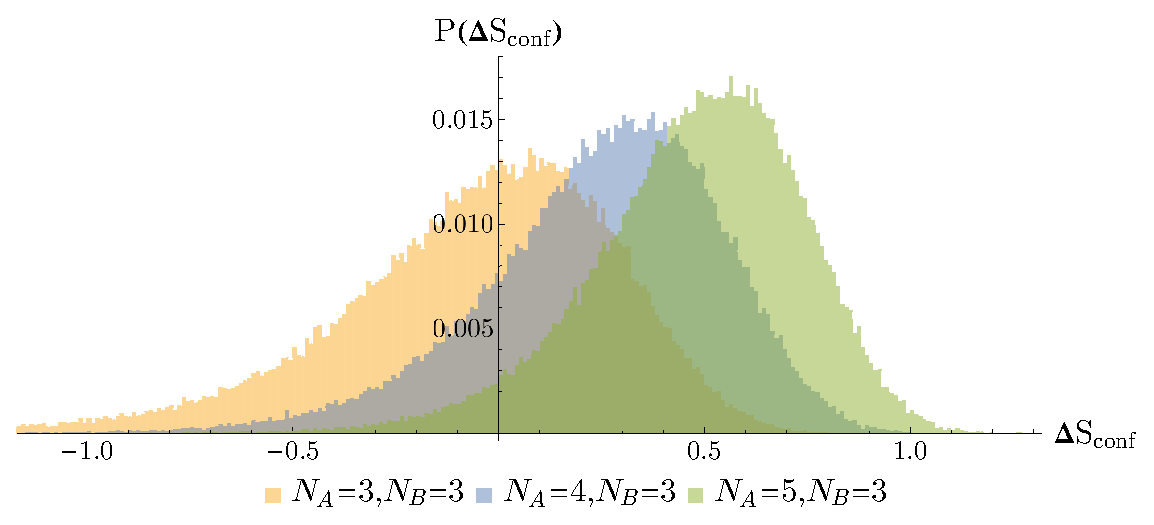
\includegraphics[width=23cm]{Figure2.eps} \caption{Probability distributions of change of entropy ($k_B =1$) in transitions between $N_A$ initial and $N_B$ final macrostates, calculations performed for $N=10^5$ random matrices.}
\label{Fig2} 
\end{figure}
\end{minipage}
\vspace{-0.5cm} 

Those results suggest that if our knowledge about the system stays in tact (no change in number of macroscopic states), then entropy most likely will not change (yellow graph from figure \ref{Fig2}). More importantly:

\vspace{0.6cm} 
\begin{tcolorbox}[colframe=green!500!white,colback=white!50!white,boxrule=3pt]
\textbf{Observation \#1a}: The preferred direction (higher entropy change) correlates with the fall in number of macroscopic (discernible) states and with growth of their microscopic realizations. In other words: The spontaneous direction of change is associated with an increasing number of inaccessible degrees of freedom.
\end{tcolorbox}


\vspace{0.6cm} 
\begin{tcolorbox}[colframe=green!500!white,colback=white!50!white,boxrule=3pt]
\textbf{Observation \#1b}: The obtained distributions of change in configurational entropy are shifted only by the chosen numbers of initial and final macroscopic states and \textit{not} by the \textit{total} number of microstates.
\end{tcolorbox}

Comparison of the forward (spontaneous) to backward (non-spontaneous) distribution:

\begin{minipage}[b]{22.0cm}
\centering
\begin{figure}[ht!]
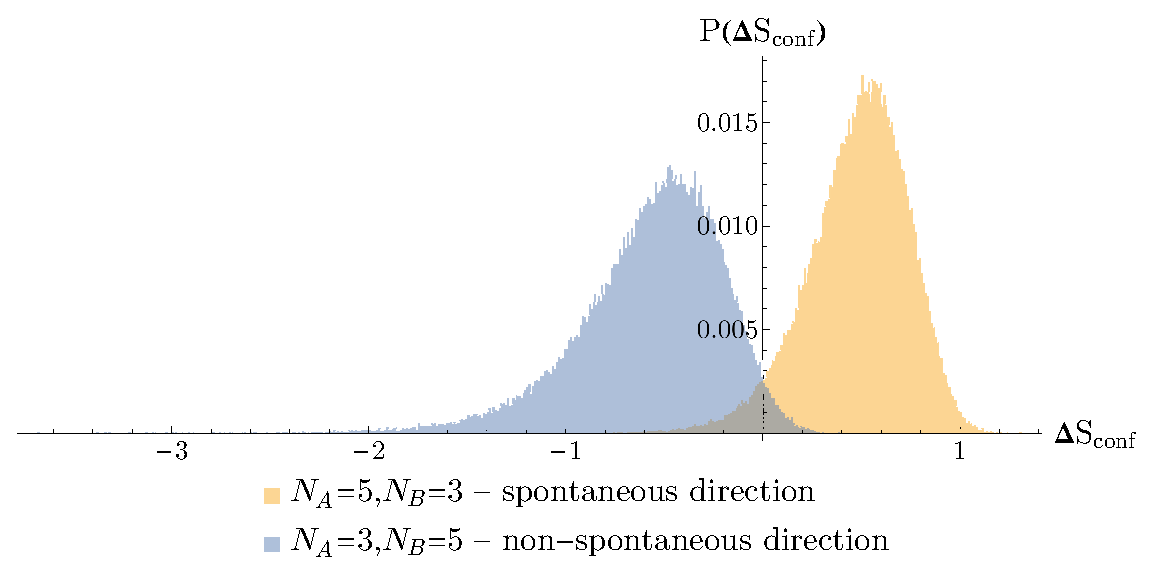
\includegraphics[width=22cm]{Figure3.eps} 
%\caption{Probability distributions of entropy produced ($k_B =1$) in transitions between $N_A$ initial and $N_B$ final macrostates, calculations performed for $N=10^5$ random matrices.}
\end{figure}
\end{minipage}
%\vspace{-1.0cm} 
\begin{minipage}[b]{23.0cm}
\centering
\begin{figure}[ht!]
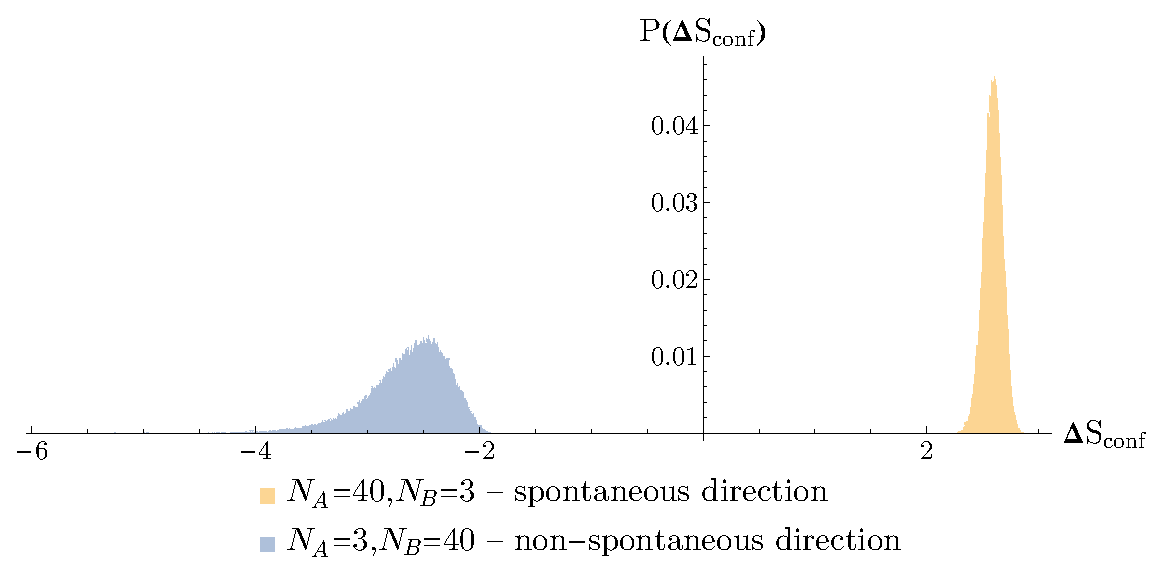
\includegraphics[width=23cm]{Figure4.eps} \caption{Probability distributions of change of entropy in transitions between $N_A$ initial and $N_B$ final macrostates and the reverse scenarios.}
\label{Fig4} 
\end{figure}
\end{minipage}

\vspace{0.3cm} 

\begin{tcolorbox}[colframe=green!500!white,colback=white!50!white,boxrule=3pt]
\textbf{Observation \#2}: The non-spontaneous direction of change is associated with wider distributions of entropy change.
\end{tcolorbox}

\begin{minipage}[b]{23.0cm}
\centering
\begin{figure}[ht!]

\includegraphics[width=23cm]{Figure5.eps} \caption{Comparison of uniform and gaussian distributions of 'transition' matrix $K_{ij}$ entries.}
\label{Fig2} 
\end{figure}
\end{minipage}
\vspace{-0.5cm} 

\begin{tcolorbox}[colframe=green!500!white,colback=white!50!white,boxrule=3pt]
\textbf{Observation \#3}: The change in distributions of entries does not change the universal character of forward versus backward transitions mentioned in Observation \#2.
\end{tcolorbox}
\vspace{2.8cm}
\begin{displaymath}
\end{displaymath}
\end{flushleft}
\columnbreak

\section{Relation to the Crooks Fluctuation Theorem}
\vspace{-1.0cm} 
\begin{minipage}[b]{22.0cm}
\centering
\begin{figure}[ht!]
 \includegraphics[clip, trim=1.0cm 19.3cm 11.0cm 2.1cm, width=20cm]{verification.pdf}
 \caption{Result obtained during experimental verification of Crooks Fluctuation theorem in the RNA folding/unfolding experiment \cite{Collin:2005fxa}}
\end{figure}
\end{minipage}
%\begin{figure}[ht!]
% \includegraphics[clip, trim=10.5cm 19.5cm 1.0cm 2.1cm, width=20cm]{verification.pdf}
%\label{Fig5} 
%\end{figure}
\begin{flushleft}
\vspace{-1.0cm} 
The distributions from the experiment look very similar to the obtained here, except for the mirror reflection and the values on the x axis.
%\vspace{0.5cm} 

\begin{tcolorbox}[colframe=yellow!500!white,colback=white!50!white,boxrule=3pt]
\textbf{Question}: Can we use this Bayesian relation to shed light on the distributions obtained in the experimental verifications of Crooks Fluctuation Theorem like \cite{Collin:2005fxa}? 
\end{tcolorbox}
\vspace{-0.5cm} 
Indeed, we can. However, to answer this question precisely, we need to realize that in Crooks fluctuation theorem the number of available microscopic states changes during the experiment (energy is provided to the system). 
\vspace{0.5cm} 

Here, the other hand, the number of microscopic states stays constant for a given matrix size. We can however, choose a different (higher) number of macroscopic final states in the non-spontaneous direction to emulate the increase in number of microscopic states ($\Delta E > 0$ in equation (\ref{ConfEntropy})), obtaining:

%\vspace{0.5cm}
%\begin{equation}
%  \Delta S = \frac{\Delta E - \Delta F}{T}
%\end{equation}

\begin{minipage}[b]{22.0cm}
\centering
\begin{figure}[ht!]
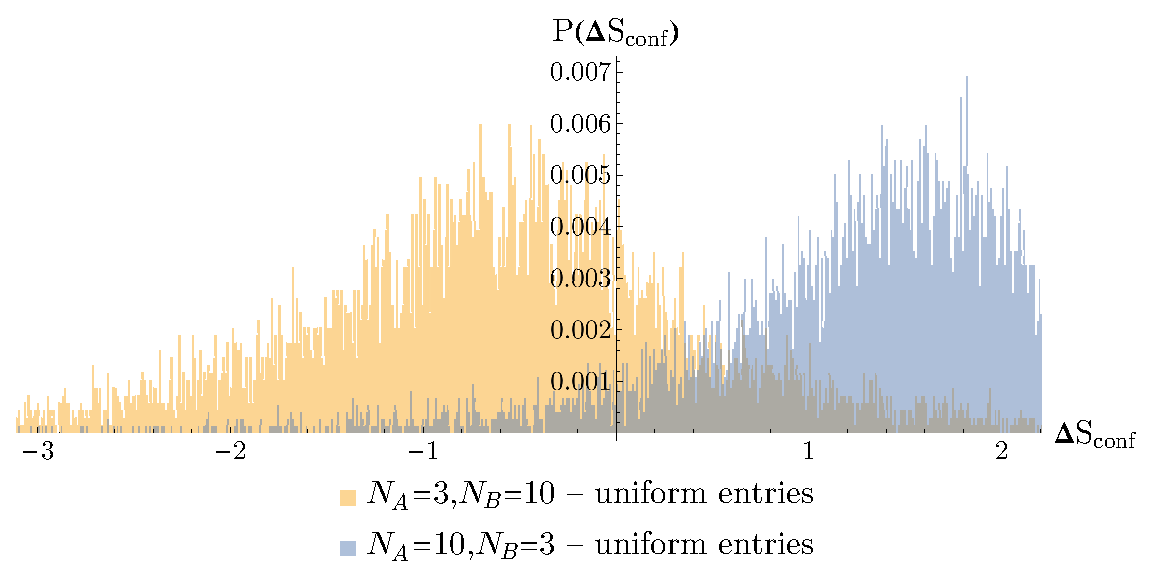
\includegraphics[width=22cm]{Figure6.eps} 
%\caption{Probability distributions of entropy produced ($k_B =1$) in transitions between $N_A$ initial and $N_B$ final macrostates, calculations performed for $N=10^5$ random matrices.}
\end{figure}
\end{minipage}
%\vspace{-1.0cm} 
\begin{minipage}[b]{23.0cm}
\centering
\begin{figure}[ht!]
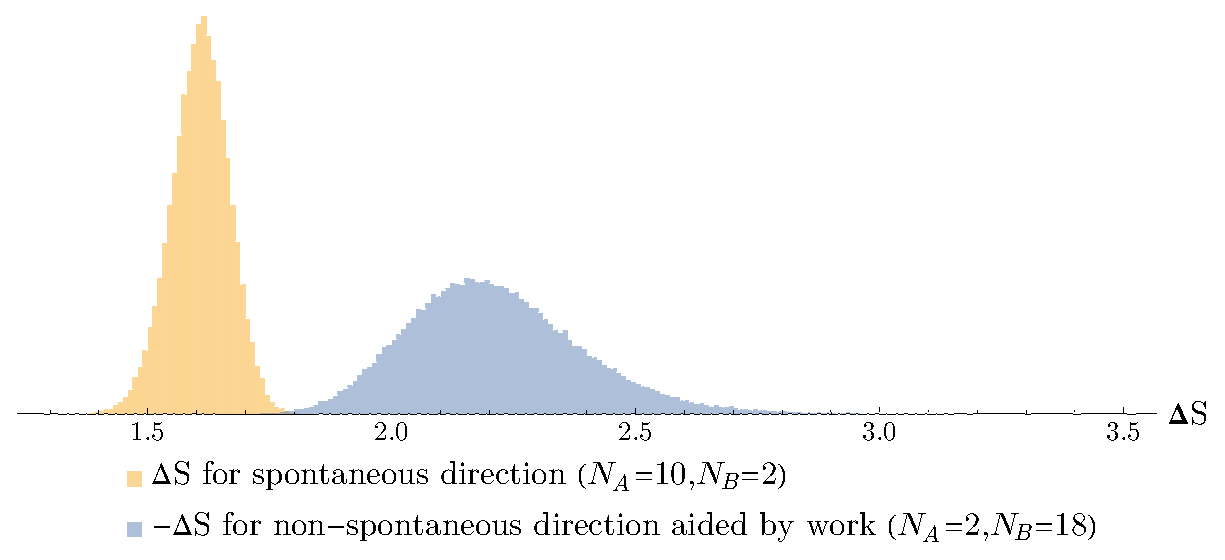
\includegraphics[width=23cm]{Figure7.eps} \caption{Probability distributions of change of entropy for spontaneous and non-spontaneous work aided transitions}
\label{Fig4} 
\end{figure}
\end{minipage}
\vspace{-1.0cm} 
\begin{tcolorbox}[colframe=green!500!white,colback=white!50!white,boxrule=3pt]
\textbf{Observation \#4}: The gap between the obtained distributions grows with the amount of work (energy) put into the system.
\end{tcolorbox}

Consistent with the results obtained in the experiment:

\end{flushleft}

\begin{minipage}[b]{22.0cm}
\centering
\begin{figure}[ht!]
 \includegraphics[clip, trim=10.0cm 4.1cm 2.0cm 17.7cm, width=20cm]{verification2.pdf}
 \caption{Result for different forces applied during the RNA folding/unfolding experiment \cite{Collin:2005fxa}}
\end{figure}
\end{minipage}
%\bibliographystyle{plain}
%\begin{thebibliography}{1}
\begin{small}
\vspace{-3.0cm}
\bibliographystyle{ieeetr}
\bibliography{Refs}
\begin{displaymath}
.
\end{displaymath}
\end{small}
\begin{displaymath}
.
\end{displaymath}
\end{multicols}
\end{document}